
\section{Examples for the Import of Contributions}

The content within the following sections is purely generated via RDFtex's import functionality.

\subsection{Dataset Import}


\begin{dataset}
SciERC~\cite{DBLP:conf/emnlp/LuanHOH18}\\
Domain: Artificial Intelligence\\
Description: ``Our dataset (called SciERC) includes annotations for scientific entities, their relations, and coreference clusters for 500 scientific abstracts."~\cite{DBLP:conf/emnlp/LuanHOH18}
\label{dataset:scierc}
\end{dataset}

\Cref{dataset:scierc} shows an imported dataset.

\subsection{Definition Import}


\begin{definition}
\label{def:knowledge-graph}
A knowledge graph acquires and integrates information into an ontology and applies a reasoner to derive new knowledge.\normalfont{~\cite{DBLP:conf/i-semantics/EhrlingerW16}}
\end{definition}

\Cref{def:knowledge-graph} shows an imported definition.

\subsection{Experimental Result Import}

\subsection{Figure Import}


\begin{figure}[htb!]
\centering
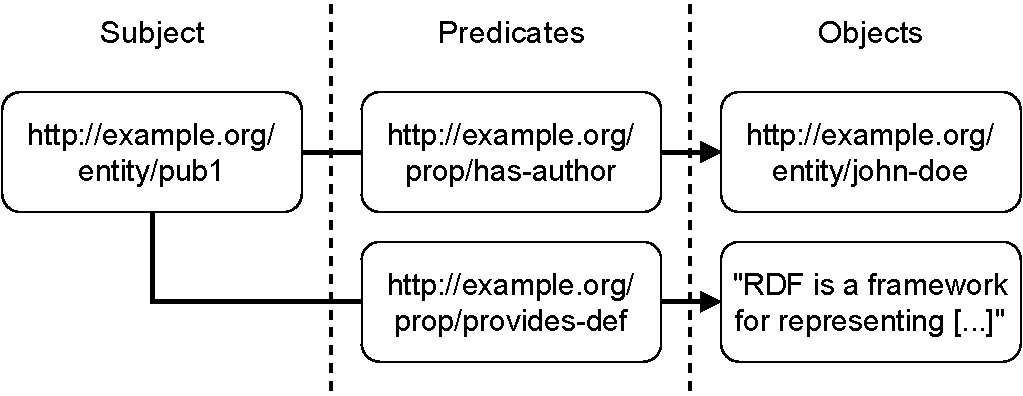
\includegraphics[max width=0.7\columnwidth]{./figures/triple_example}
\caption{A simple exemplary knowledge graph consisting of two RDF triples. The upper triple provides contextual information, the lower triple contentual information of the publication \emph{{pub1}}. All non-literal triple members are identified using IRIs. (Figure and caption adopted from~\cite{Martin21}.)}
\label{fig:contentual-contextual}
\end{figure}

\Cref{fig:contentual-contextual} shows an imported figure.

\subsection{Software Import}


\begin{software}
Prot{\'{e}}g{\'{e}}-2000~\cite{DBLP:conf/amia/NoyCFKTVM03}\\
Available at: \url{https://protege.stanford.edu}\\
Description: ``Prot\'{e}g\'{e}-2000 is an open-source tool that assists users in the construction of large electronic knowledge bases. It has an intuitive user interface that enables developers to create and edit domain ontologies. Numerous plugins provide alternative visualization mechanisms, enable management of multiple ontologies, allow the use of inference engines and problem solvers with Prot\'{e}g\'{e} ontologies, and provide other functionality."~\cite{DBLP:conf/amia/NoyCFKTVM03}
\label{software:protege}
\end{software}

\Cref{software:protege} shows an imported software.


